% design_cut.tex — ONE source, ONE rendered SVG (design_cut.svg), embedded in ../modules.md.
%
% The claim: the SAME three modules under TWO cuts.  Nothing about mod2 changes between the two
% panels — only where the boundary was drawn, and therefore which realization hook is consulted.
%
% Render: bash render.sh   (MiKTeX pdflatex -> PDF -> dvisvgm --pdf -> SVG)
\documentclass[tikz,border=4pt]{standalone}
\usepackage{tikz}
\usetikzlibrary{arrows.meta,positioning,calc,fit,backgrounds}

% Theme-neutral palette: the SVG is viewed on both light and dark docs pages, so the fills stay
% pale and every stroke/label is explicit rather than inherited.
\definecolor{dutfill}{HTML}{DCE9F7}
\definecolor{dutline}{HTML}{2C6FB5}
\definecolor{bfmfill}{HTML}{F2E6D0}
\definecolor{bfmline}{HTML}{9A6B1F}
\definecolor{inkgray}{HTML}{444444}

\begin{document}
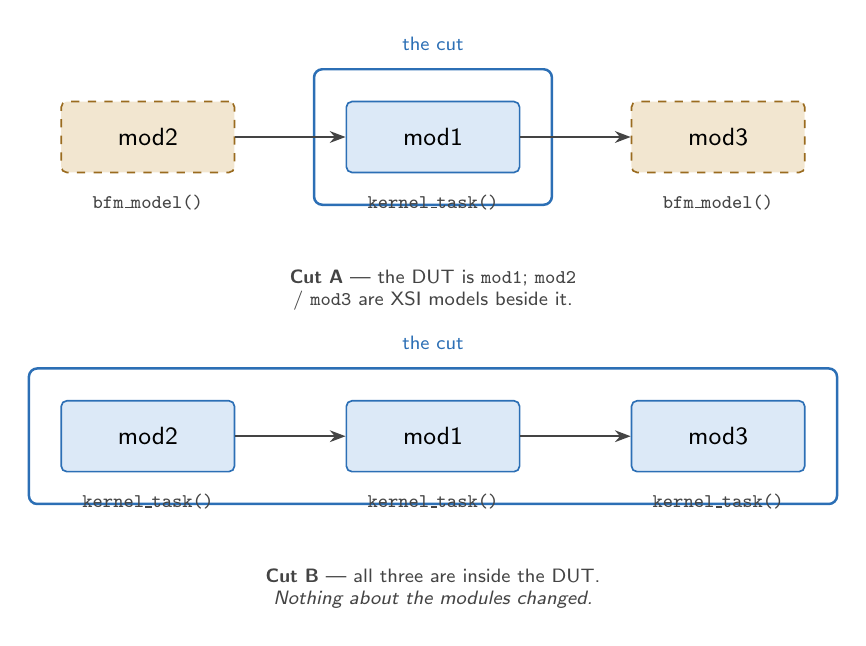
\begin{tikzpicture}[
  font=\sffamily\small,
  mod/.style   = {draw, rounded corners=2pt, minimum width=22mm, minimum height=9mm,
                  align=center, line width=0.6pt},
  inside/.style= {mod, fill=dutfill, draw=dutline},
  outside/.style={mod, fill=bfmfill, draw=bfmline, dashed},
  flow/.style  = {-{Stealth[length=2mm]}, line width=0.7pt, draw=inkgray},
  cut/.style   = {draw=dutline, line width=0.9pt, rounded corners=3pt},
  lbl/.style   = {font=\sffamily\scriptsize, text=inkgray},
  hook/.style  = {font=\ttfamily\scriptsize, text=inkgray},
]

% ---------- panel A : cut around mod1 alone -------------------------------------------------
\node[inside]  (a1) {mod1};
\node[outside, left=14mm of a1]  (a0) {mod2};
\node[outside, right=14mm of a1] (a2) {mod3};
\draw[flow] (a0) -- (a1);
\draw[flow] (a1) -- (a2);
\begin{scope}[on background layer]
  \node[cut, fit=(a1), inner sep=4mm] (acut) {};
\end{scope}
\node[lbl, text=dutline, above=1mm of acut.north] {the cut};
\node[hook, below=1.5mm of a1.south]  {kernel\_task()};
\node[hook, below=1.5mm of a0.south]  {bfm\_model()};
\node[hook, below=1.5mm of a2.south]  {bfm\_model()};
\node[lbl, below=11mm of a1.south, text width=62mm, align=center]
     {\textbf{Cut A} — the DUT is \texttt{mod1}; \texttt{mod2} / \texttt{mod3} are XSI models beside it.};

% ---------- panel B : cut around all three --------------------------------------------------
\begin{scope}[yshift=-38mm]
  \node[inside] (b1) {mod1};
  \node[inside, left=14mm of b1]  (b0) {mod2};
  \node[inside, right=14mm of b1] (b2) {mod3};
  \draw[flow] (b0) -- (b1);
  \draw[flow] (b1) -- (b2);
  \begin{scope}[on background layer]
    \node[cut, fit=(b0)(b1)(b2), inner sep=4mm] (bcut) {};
  \end{scope}
  \node[lbl, text=dutline, above=1mm of bcut.north] {the cut};
  \node[hook, below=1.5mm of b0.south] {kernel\_task()};
  \node[hook, below=1.5mm of b1.south] {kernel\_task()};
  \node[hook, below=1.5mm of b2.south] {kernel\_task()};
  \node[lbl, below=11mm of b1.south, text width=72mm, align=center]
       {\textbf{Cut B} — all three are inside the DUT. \emph{Nothing about the modules changed.}};
\end{scope}

\end{tikzpicture}
\end{document}
